\section{Hintergrund}\label{Hintergrund}
Ein Compiler hat im Allgemeinen zwei Phasen: das Frontemd und das Backend. In diesem Projekt soll ein Frontend f�r einen Compiler erstellt werden.
In diesem Frontend wird ein sogenannter Logdatei-Parser eingesetzt. Er liest eine Eingabe im Agilent-Logformat und erstellt daraus ein Syntax-Baum in einem gegebenen Zwischenformat.
In einem Folgeprojekt wird ein Compiler-Backend erstellt, dass den vom Frontend erzeugten Zwischencode nimmt und daraus die gew�nschte Ausgabe in einem Zielformat schreibt. In Abbildung \ref{fig:BigPicture} auf Seite \pageref{fig:BigPicture} ist die Umgebung dargestellt, in der der Log-Parser verwendet wird.

Da das Agilent-Logformat nur halbformal in einer pdf-Datei beschrieben ist und es keine formale Grammatik f�r das Format gibt, k�nnen keine Parsergeneratoren wie JavaCC oder yacc eingesetzt werden, sondern es wird hier f�r das Agilent-Logformat ein Parser von Hand geschrieben.

\begin{figure}[htp]
\centering
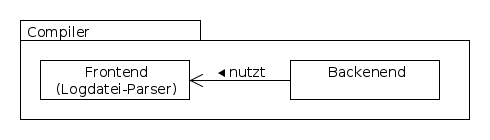
\includegraphics[width=0.8\textwidth]{Ingo/Bilder/BigPicture.png}
\caption{Big Picture}
\label{fig:BigPicture}
\end{figure}